\documentclass[a4paper]{article}

\usepackage[utf8]{inputenc}
\usepackage[dutch]{babel}
\usepackage{fancyhdr} %Why the hell does the KU Leuven not have it's own latex header package but the KULAK does?
\usepackage{amsmath}
\usepackage{graphicx}
\usepackage[space]{grffile}
\usepackage{authblk}
\graphicspath{{D:/Jonas/Google Drive/KULeuven3/NumeriekeModelleringBenadering/Practicum/images/}}

\pagestyle{plain}
\title{Numerieke Modellering \& Benadering Practicum}
\author{Dennis Debree}
\author{Jonas Bertels}
\affil{KU Leuven Departement Computerwetenschappen}


\begin{document}
\maketitle
\section{Bivariate Veelterm Benadering}
\subsection{Inleiding}
Voor het vak numerieke modellering en benadering aan de KU Leuven werd de opdracht gegeven een bivariate veelterm benadering te implementeren in MATLAB. Deze benadering werd dan gebruikt om enkele 2 dimensionale oppervlakken te benaderen. Dit verslag geeft een visueel overzicht van de benaderingen en hun oppervlak en van de nauwkeurigheid van de benadering afhankelijk van de graad van de benaderende veelterm.
\subsection{De basisfunctie}
\begin{verbatim}
function C = kkb(x, y, F, m, n)
Afull = fliplr(vander(x));
Bfull = fliplr(vander(y));
C =  Bfull(:, 1:n)\F*pinv((Afull(:, 1:m)))';
end
\end{verbatim}
Deze functie creëert eerst de A en B Vandermonde matrices om hieruit de x en y waarden te halen. Daarna wordt uit deze A en B matrices de F matrix berekent door eerst de graad van de A en B matrices te verkorten tot m en n en hierna C te bereken door de formule $C = B^{+}F(A^{+})^{T}$. Deze formule werd als volgt afgeleid:\\
We proberen het volgende te minimaliseren:
\begin{equation}
C = B^{+}F(A^{+})^{T} \label{solution}
\end{equation}
Om dit te doen moet $\Gamma c = f$ of $\Gamma^{+} \vec(F) = C$ en aangezien $\Gamma = A\otimes B$ geldt:
\begin{equation}
\text{vec}(C) = (A\otimes B)^{+}\text{vec}(F) = (A^{+}\otimes B^{+})\text{vec}(F) = \text{vec}(B^{+}F(A^{+})^{T})   \label{singleInverse}\\
\end{equation}
(Omdat we weten dat:)
\begin{equation}
(A\otimes B)^{+} = A^{+} \otimes B^{+} \label{distribution}\\
\end{equation}
\begin{equation}
(A\otimes B)\text{vec}(F) = \text{vec}(BFA^{T}) \label{transformation}\\
\end{equation}

Oorspronkelijk werd \eqref{singleInverse} gebruikt in plaats van \eqref{solution} omdat we dachten dat \eqref{singleInverse} ons toeliet om slechts 1 inverse matrix uit te rekenen in plaats van 2 en zo de hoeveelheid benodigd werk doet dalen. Dit was natuurlijk fout omdat $A\otimes B$ dimensies heeft die het product zijn van de dimensies van de A en B matrices. Toen de functiebenadering van de Etna moest gegenereerd worden bleek al snel dat het gebruik van \eqref{singleInverse} helemaal geen optimalisatie was in termen van geheugen. Het Kronecker product zorgde er namelijk voor dat matrices zo groot werden dat ze niet meer in het geheugen pasten, en dat bij kleinere waarden van $m$ en $n$ het verschillende minuten duurde voordat de matrix gegenereerd werd (dit is logisch want bij een $m = n = 25$ is $\dim(A) = 1425\times25$ en $\dim(B) = 1425\times25$ waardoor het Kronecker product een dimensie van $2030625\times625$ had).

\subsection{2 functiebenaderingen}
\begin{figure}
\caption{Functiebenadering van $\sin ((2x - 1)^{2} + 2y)$}
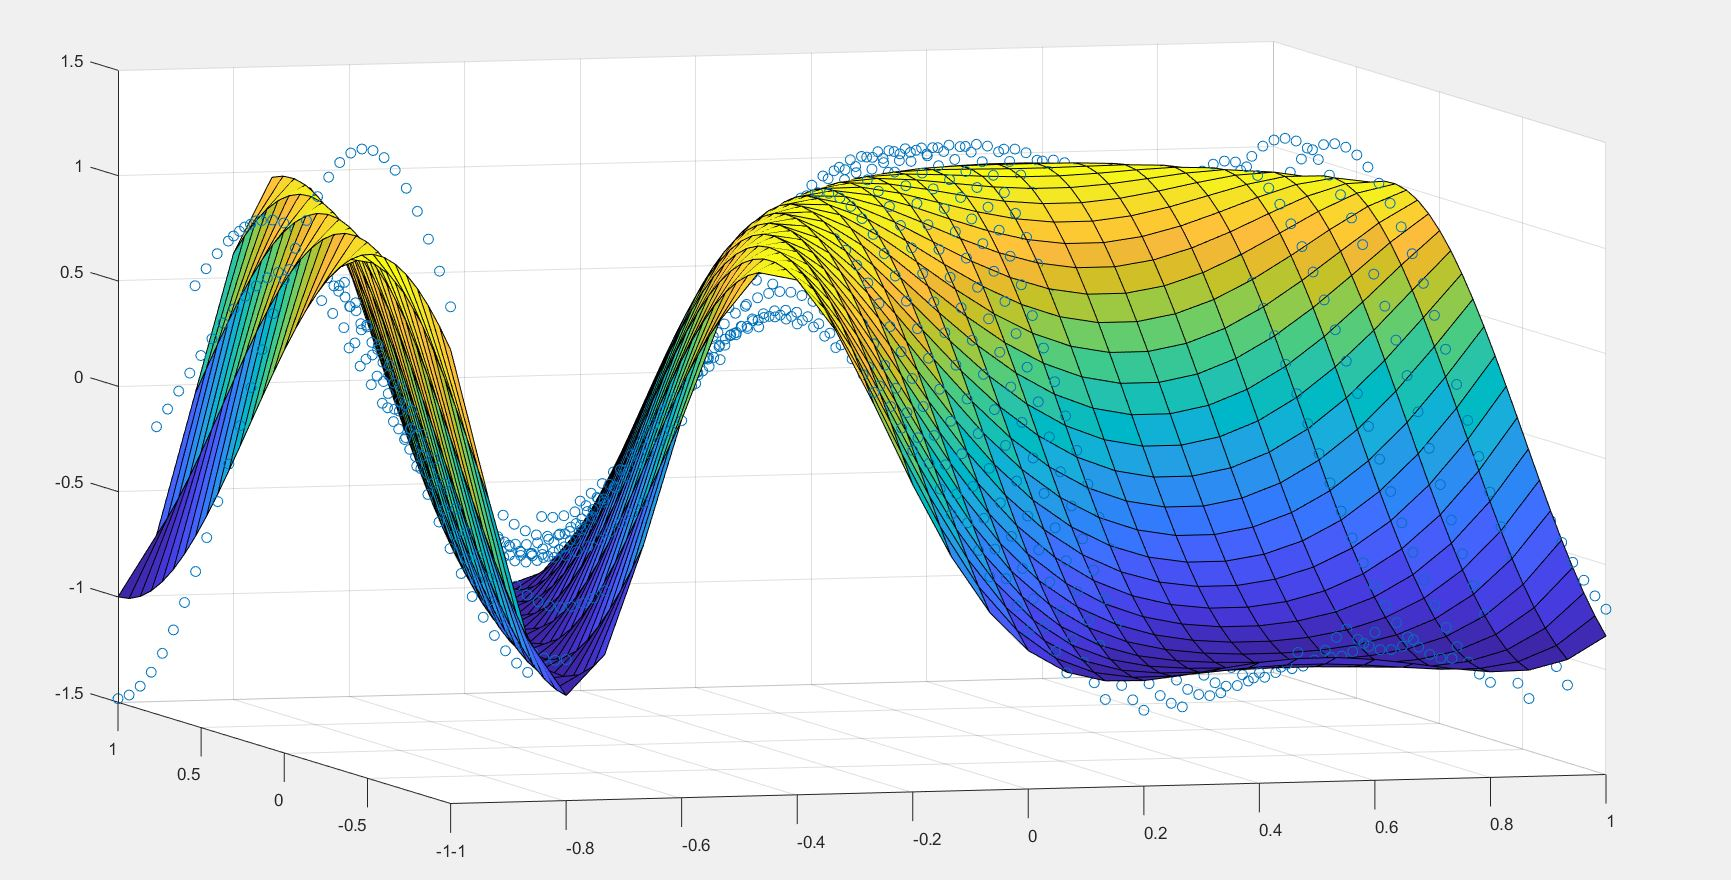
\includegraphics[width=\textwidth, height=0.3\textheight]{Excercise12Sin.JPG}
\end{figure}
\begin{figure}
\caption{Functiebenadering van de membraan functie}
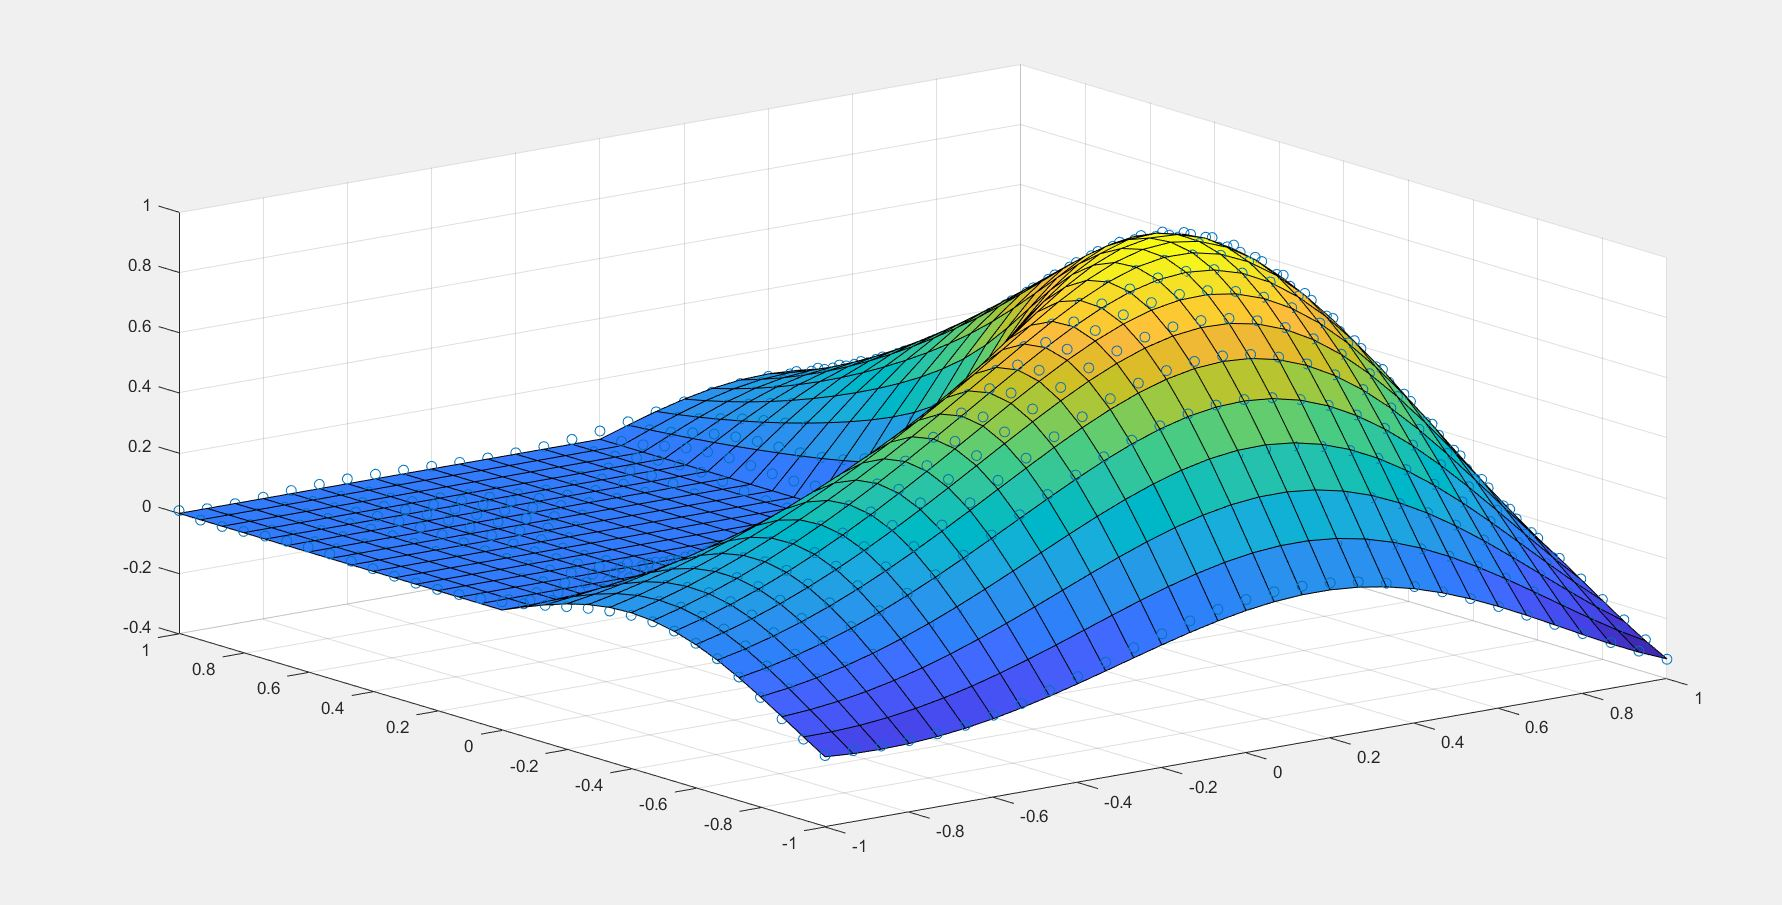
\includegraphics[width=\textwidth, height=0.3\textheight]{Excercise12Membrane.JPG}
\end{figure}
We gebruiken nu de kkb functie om enkele 2-D oppervlakken te benaderen. De gegeven functie polyval laat ons toe aan de hand van het resultaat van onze kkb-functie de benaderde waarden voor x en y te evalueren. Op Figuur 1 en Figuur 2 is de functie voorgesteld als een oppervlak en de benaderde waarden als punten (de blauwe cirkels) die boven of onder dit oppervlak verschijnen.

\subsection{De kostfunctie afhankelijk van de graad van de benaderende veelterm}
De volgende stap is het effect bepalen van de graad van de benaderende veelterm op de nauwkeurigheid van de benadering. Om dit te doen gebruikten we de volgende formule: $\sum_{i=1}^{M}\sum_{j=1}^{N}(f_{ij}-z(x_{i},y_{j}))^{2}$. Het resultaat is te zien op figuur 3.
\begin{figure}
\caption{Kostfunctie als functie van n=m}
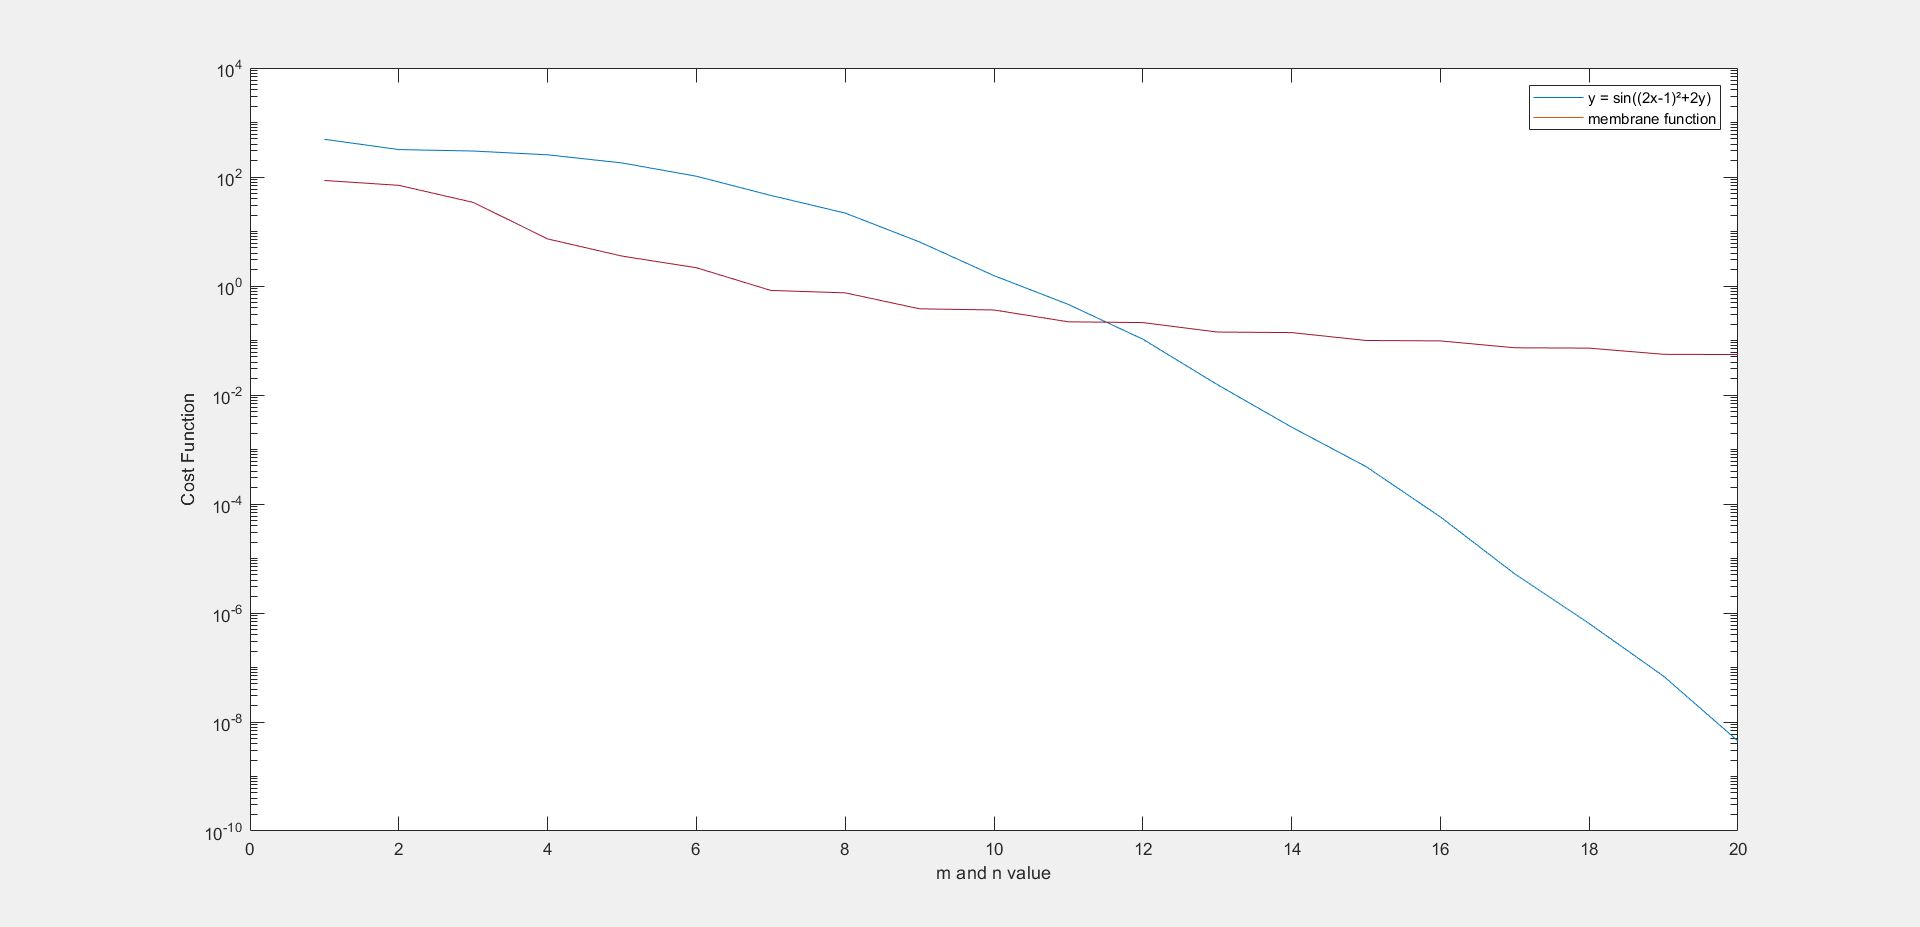
\includegraphics[width=\textwidth, height=0.3\textheight]{Excercise13.JPG}
\end{figure}
\subsection{Veeltermbenadering Etna}
De veeltermbenadering van de Etna werd op praktisch dezelfde manier geïmplementeerd als de functiebenaderingen in oefening 1.2. Zoals al eerder vermeld kwam het door deze functiebenadering dat we begrepen dat onze oorspronkelijk implementatie van kkb niet optimaal was.
\begin{figure}
\caption{De Etna volgens  ASTER Global Digital Elevation Map}
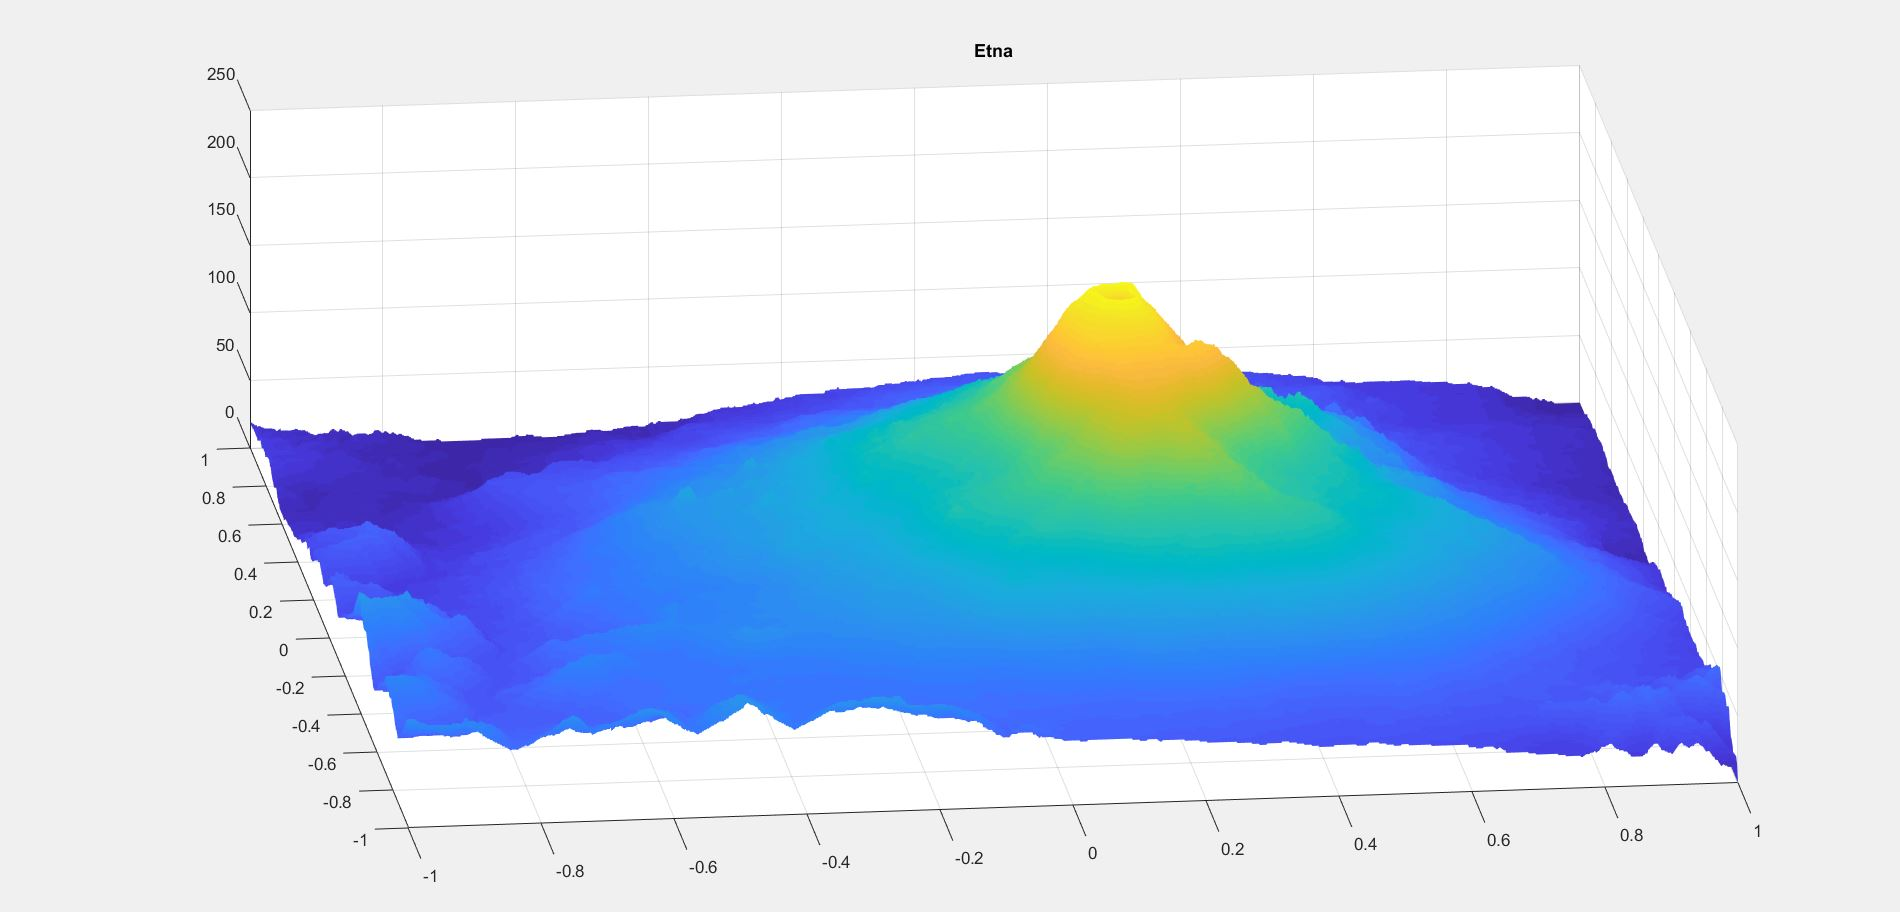
\includegraphics[width=\textwidth, height=0.3\textheight]{Excercise14Etna.JPG}
\end{figure}
\begin{figure}
\caption{Functiebenadering van de Etna met $m = n = 25$}
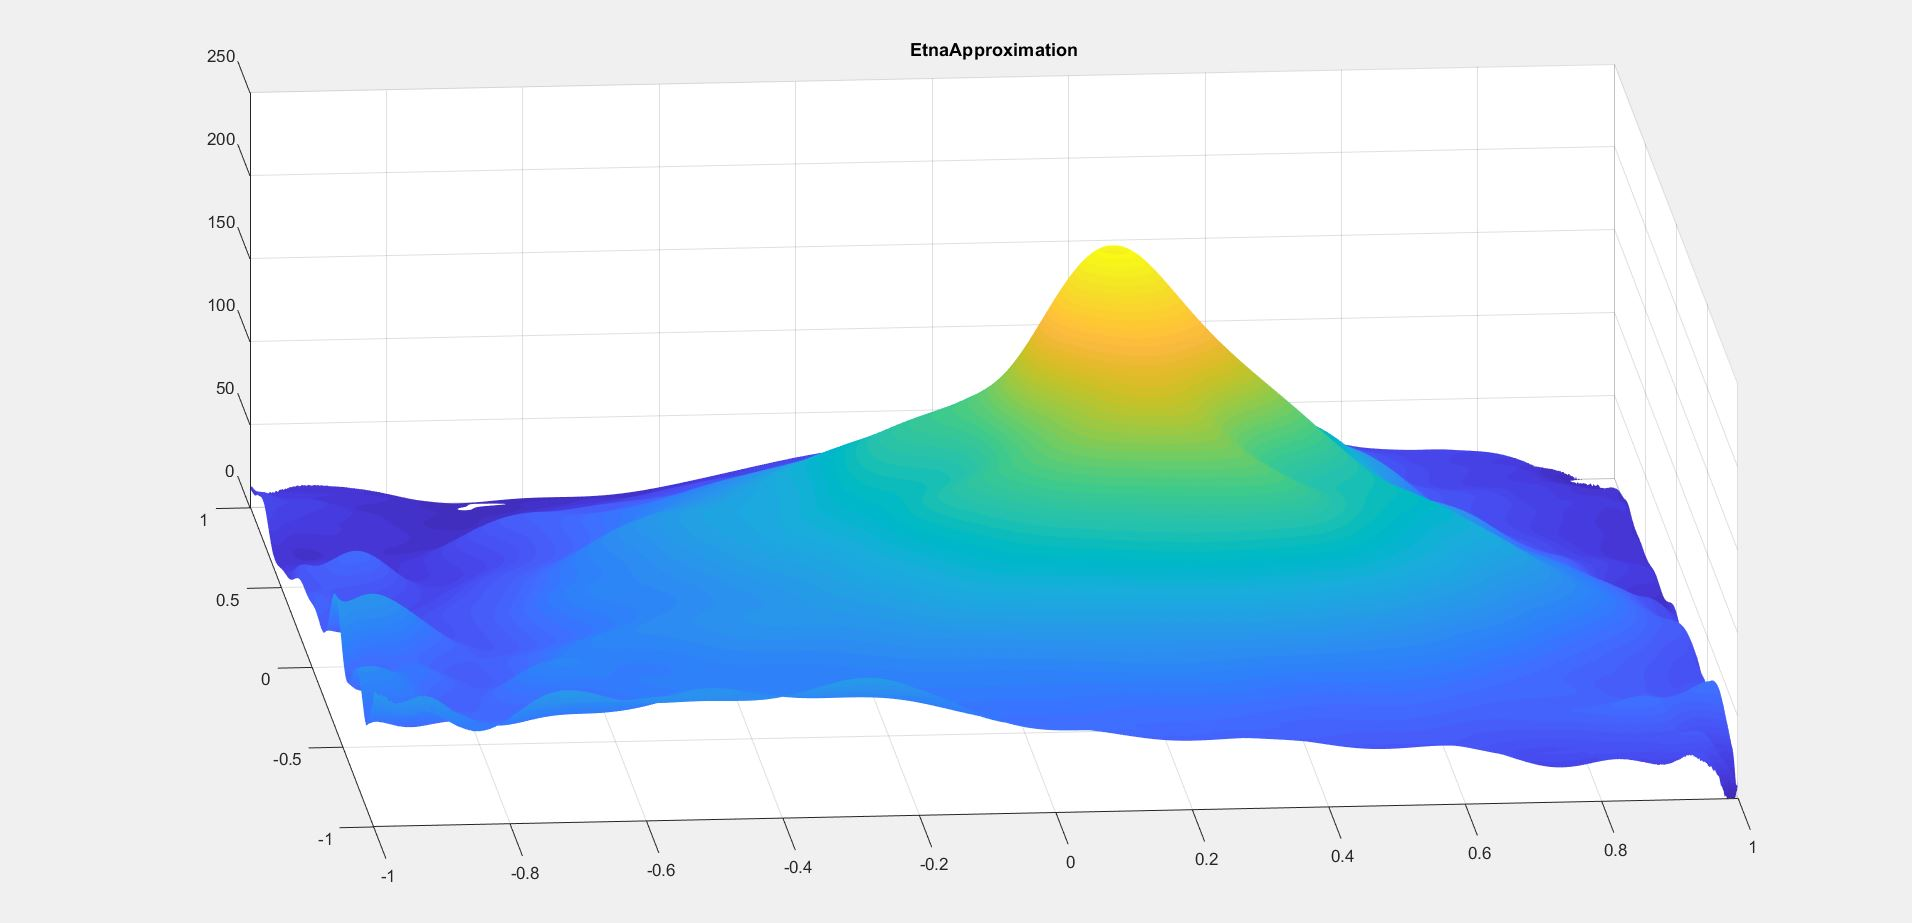
\includegraphics[width=\textwidth, height=0.3\textheight]{Excercise14EtnaBenadering.JPG}
\end{figure}
\section{Benadering via splines}
Deze opgave vroeg ons om een Matlab-functie te schrijven die een optimale interpolerende kubische spline-benadering maakt en dan deze spline evalueert in de gegeven functiewaarden. Met deze functie is het dan de bedoeling om enkele functies of krommen te benaderen. De resultaten en gebruikte werkwijzen worden in de volgende paragrafen besproken.
\subsection{Deel 1}
Als gegevens om de spline te bepalen worden alle abscissen gegeven van de te bepalen functie of krommen ($x_{0}$ tot $x_{n}$) samen met de alle functiewaarden behalve de laatste ($f_{0}$ tot $f_{n-1}$). De laatste functiewaarde moet volgens de definitie van periodieke spline gelijk zijn aan de eerste ($f_{n} = f_{0}$).\\

Voor het efficiënt oplossen van krommen waarbij meerdere splines met dezelfde abscissen bepaald moeten worden, mag de lijst van functiewaarden ook een matrix zijn, waarbij elke rij in deze matrix één set van functiewaarden bepaald.\\

Met deze gegevens kan dan volgens de theorie uit paragraaf 5.2.3 uit de cursus de matrix $A$ en vector $b$ (of matrix met in iedere kolom de vector horende bij een set gegeven functiewaarden) bepaald worden. Deze kunnen dan gebruikt worden om het stelsel $As = b$ op te lossen naar $s$, wat een vector (of matrix met in iedere kolom de vector horende bij een set functiewaarden, in dezelfde volgorde als in matrix $b$) geeft met de waarden $s''_{0}$ tot $s''_{n-1}$. Uit de definitie van periodieke splines kunnen we bepalen dat $s''_{n}$ gelijk moet zijn aan $s''_{0}$.

Hiermee bepalen we dan als laatste de constanten $c_{1}$ en $c_{2}$ voor iedere 3de-graads polynoom $p_{1}$ tot $p_{n}$ in de spline, waardoor we een vector (of matrix, met zelfde structuur als $s$) met alle $c_{1}$’s en $c_{2}$’s bekomen. Hiermee zijn alle onbekenden van onze spline benadering(en) bepaald.

Voor het evalueren van de spline-benadering gebruiken we het kenmerk van deze benadering dat iedere bepaalde 3de-graads polynoom $p_{i}$ slechts geldig is binnen het interval [$x_{i-1}$, $x_{i}$].
De abscissen voor de te bepalen functiewaarden worden gegeven in een vector $t$.
Het volstaat dus voor iedere waarde $t_{j}$ het interval te zoeken waarbij $x_{i-1} \leq t_{j} \leq x_{i}$ en dan de polynoom horende bij dit interval te evalueren in $t_{j}$. Indien meerdere splines benaderd werden, gebeurt deze evaluatie ook voor iedere spline op hetzelfde moment (eg. We berekenen de functiewaarde in $t_{j}$ voor iedere benaderde spline in 1 Matlab operatie, gezien Matlab ons toestaat operaties rechtstreeks op vectoren uit te voeren).

\subsection{Deel 2}
We gebruiken nu de functie die hierboven beschreven werd om de functie
\begin{equation}
f(x) = \sin(x) + \frac{\sin(4x)}{2}
\end{equation}
te bepalen.\\
Figuur 6 toont de benadering met 20 equidistant gekozen abscissen.
We zien hier dat voor 20 abscissen de functie vrij goed benaderd lijkt te zijn. De rode punten zijn de gegeven functiewaarden, de groene de punten geëvalueerd op de spline.
\begin{figure}
\caption{Spline Benadering met 20 abscissen}
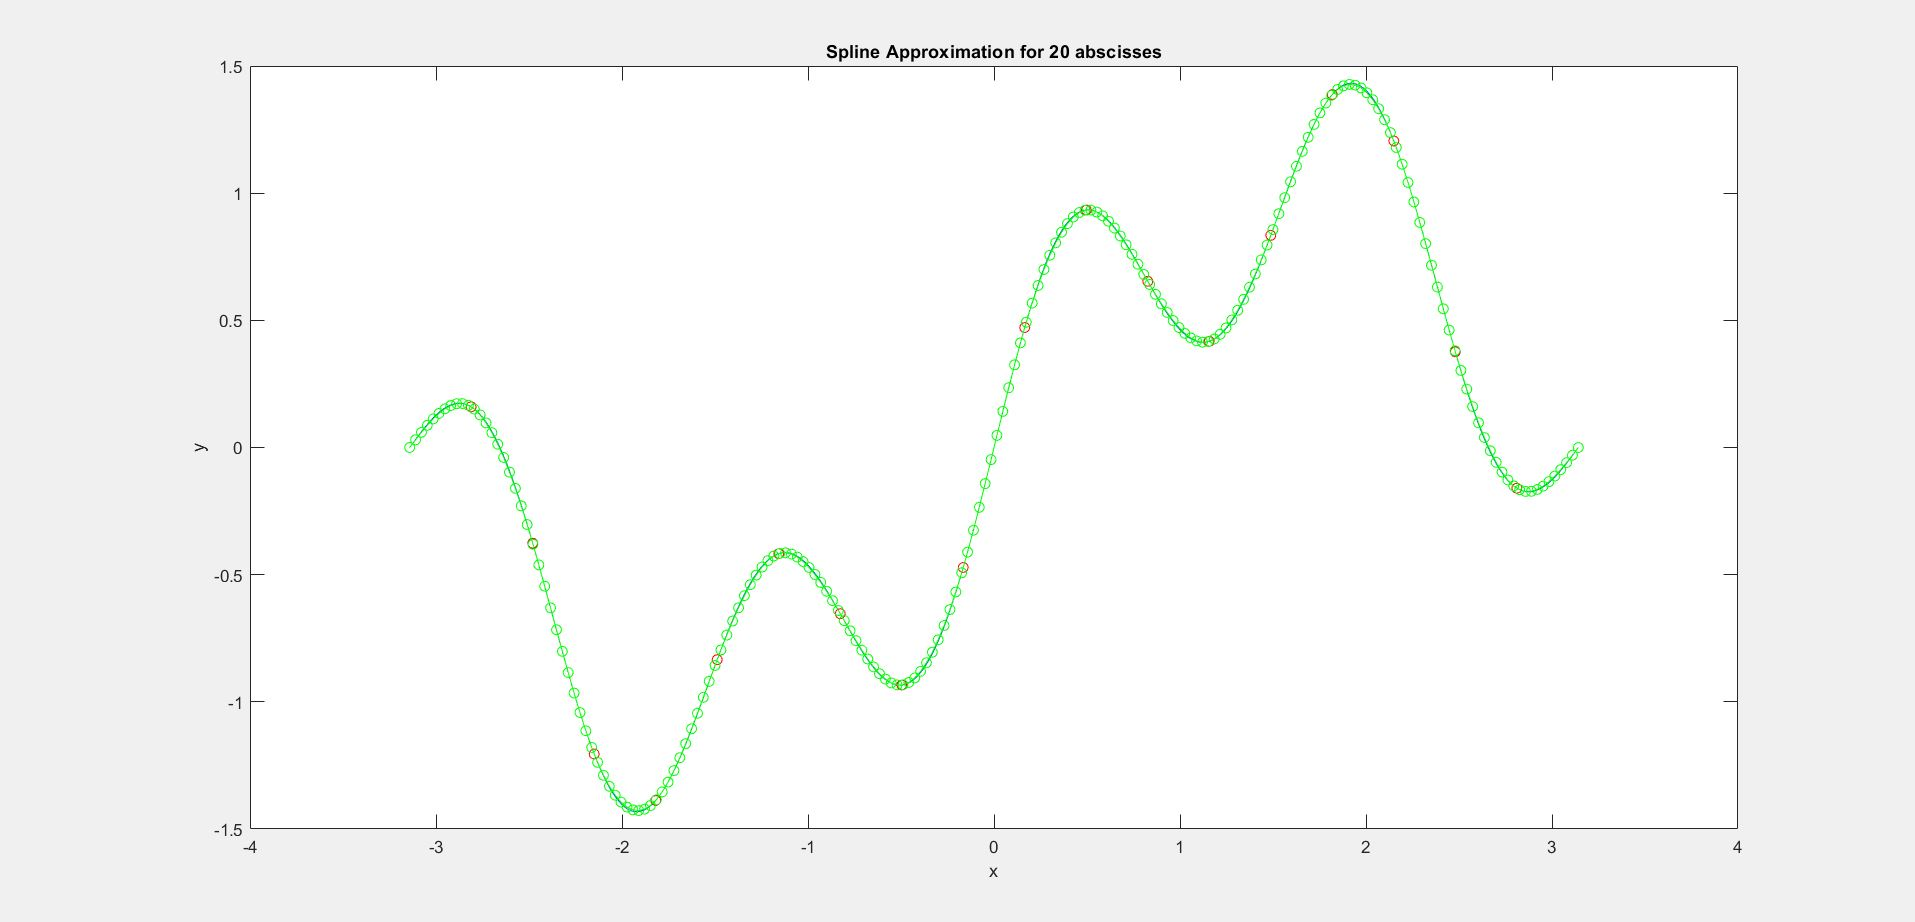
\includegraphics[width=\textwidth, height=0.3\textheight]{Excercise22SplineApprox.JPG}
\end{figure}

Figuur 7 toont de absolute fout tussen de gegeven functie en de spline benadering voor aantal abscissen gelijk aan 10 en 20 (opnieuw equidistant gekozen). We zien duidelijk dat de fouten verkleinen maar steeds oscilleren tussen de vastgelegde punten (dit zijn de nulpunten). Dit is te verwachten met een veeltermbenadering.

\begin{figure}
\caption{Absolute fout spline benadering}
	\begin{minipage}{.5\textwidth}
		\centering
		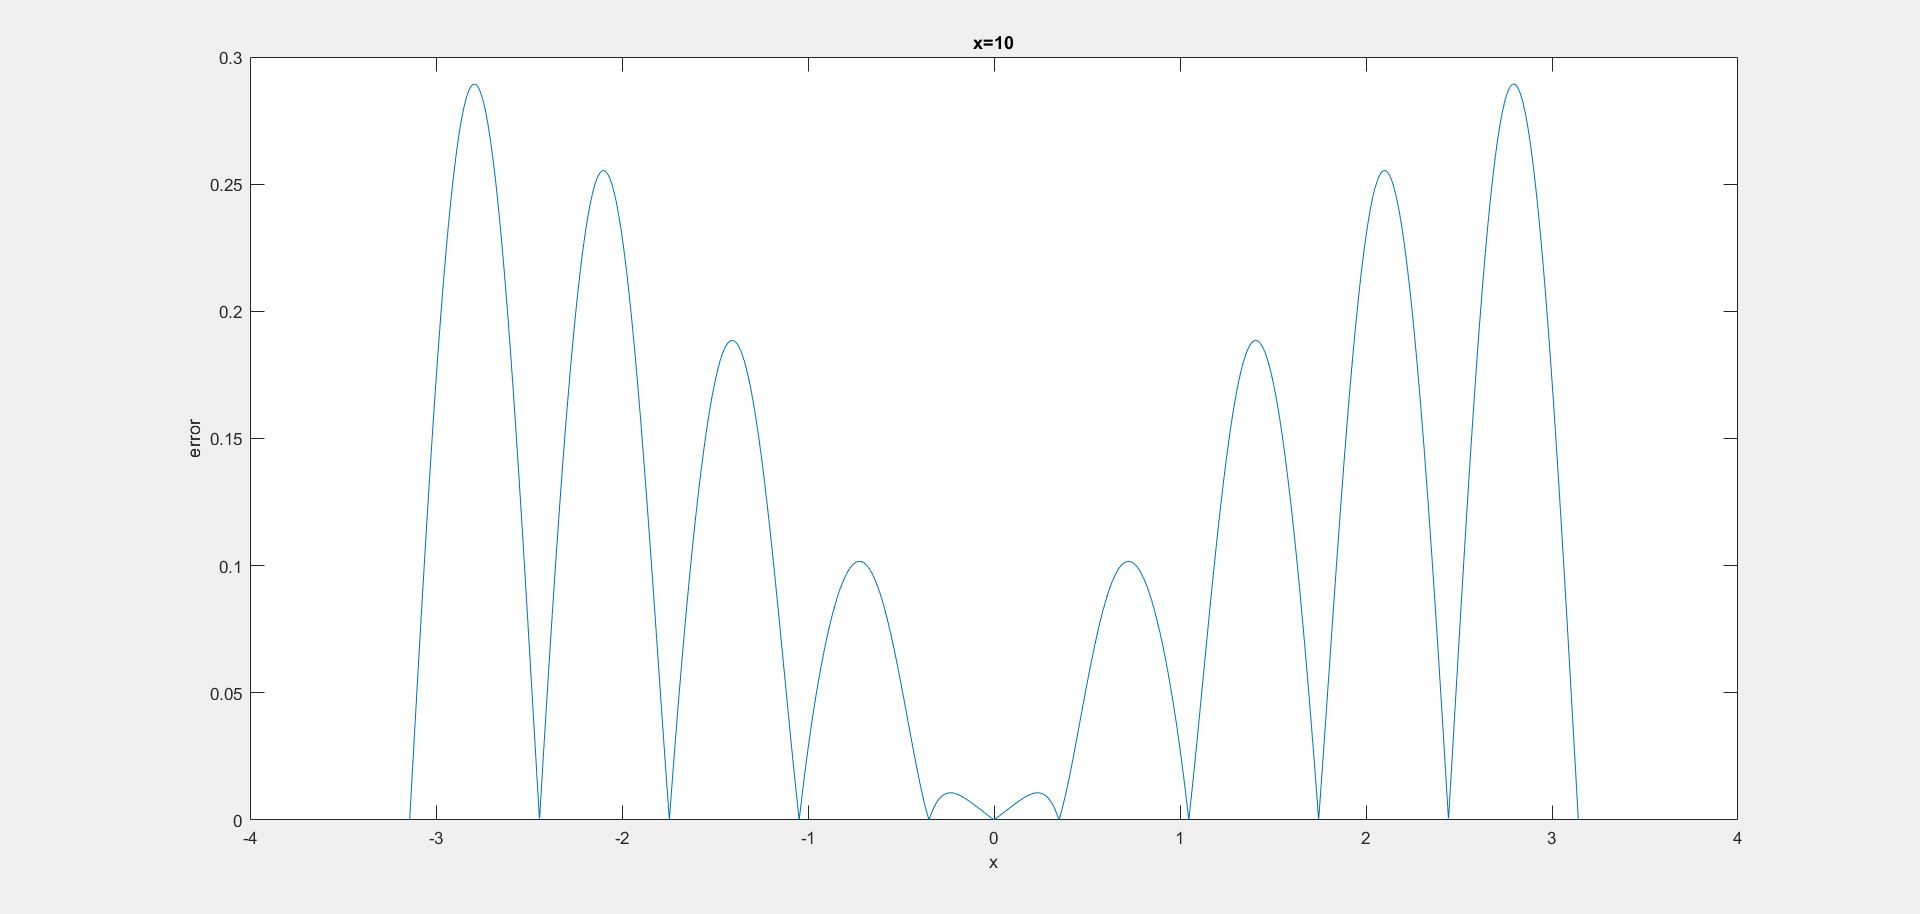
\includegraphics[width=\textwidth, height=0.2\textheight]{Excercise22AbsoluteError10.JPG}
	\end{minipage}
	\begin{minipage}{.5\textwidth}
		\centering
		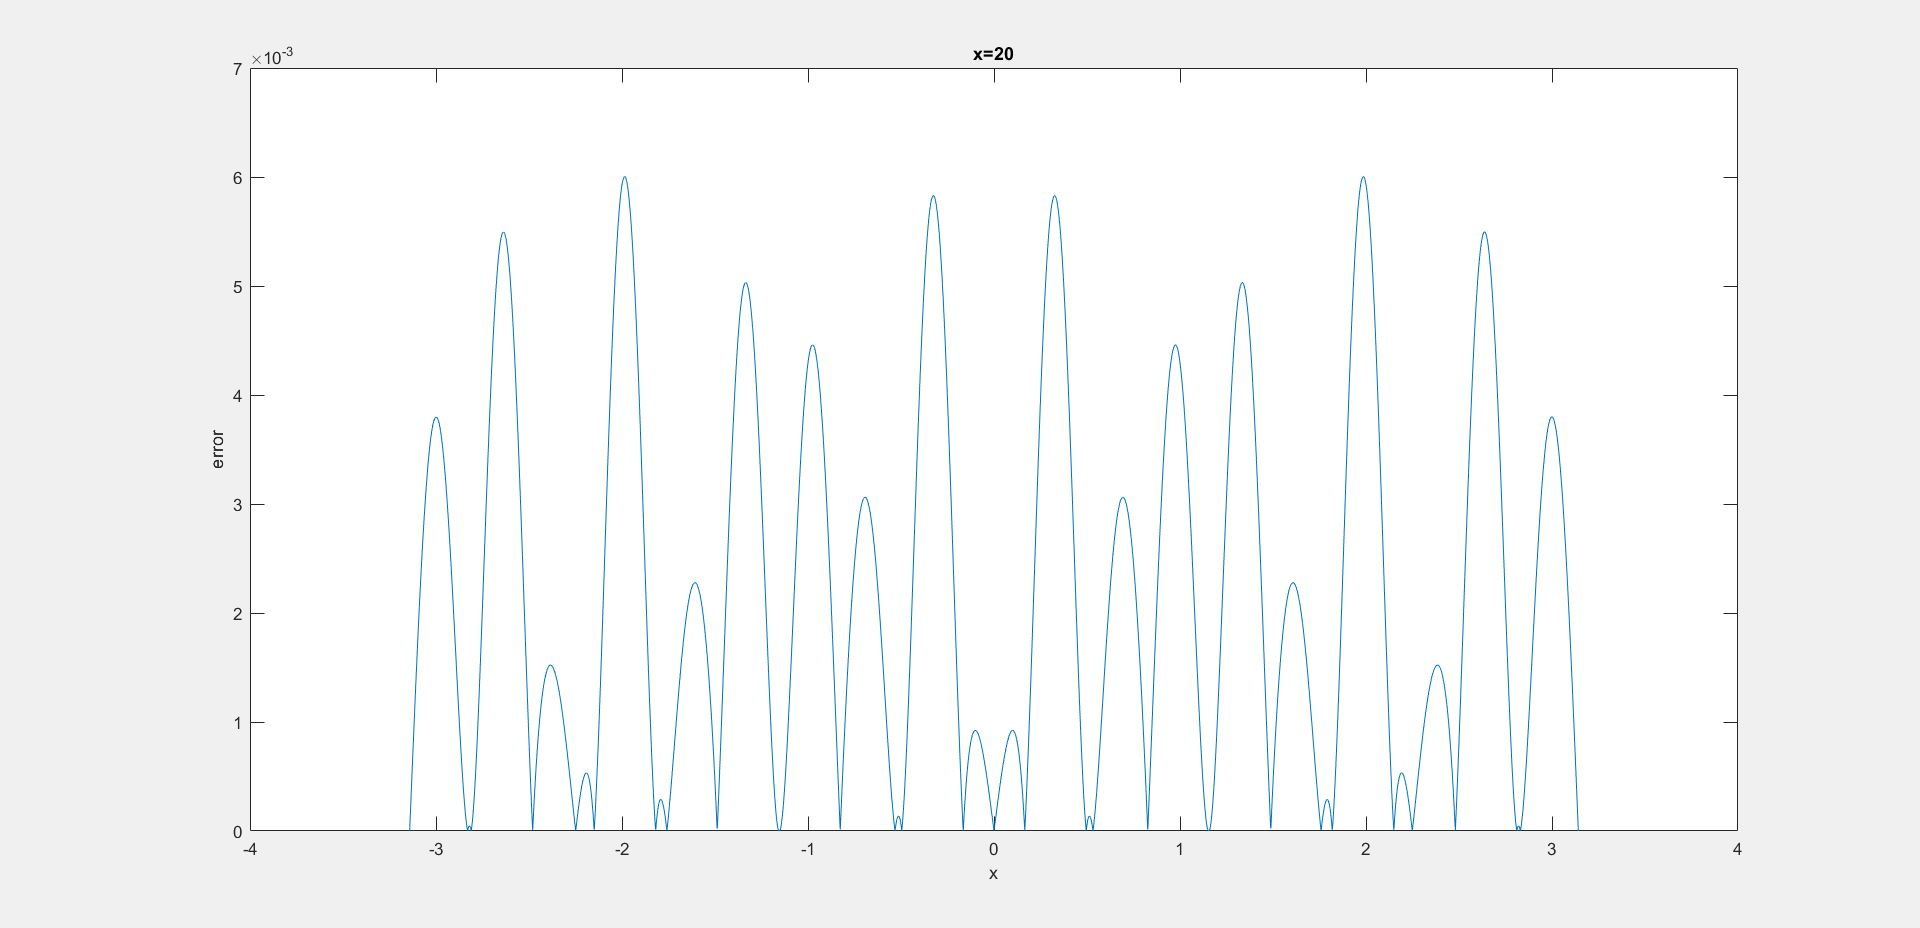
\includegraphics[width=\textwidth, height=0.2\textheight]{Excercise22AbsoluteError20.JPG}
	\end{minipage}
\end{figure}
Figuur 8 toont de maximale fout in de benadering bij een gegeven aantal abscissen, de error wordt logaritmisch geplot.
We zien dat de fout in het begin heel sterk afneemt, maar dan afzwakt. Een foutloze benadering  kan nooit bekomen worden, benaderen tot op machineprecisie nauwkeurig is misschien mogelijk maar zou zeer veel rekenwerk vergen.
\begin{figure}
\caption{Maximale fout in functie van het aantal abscissen}
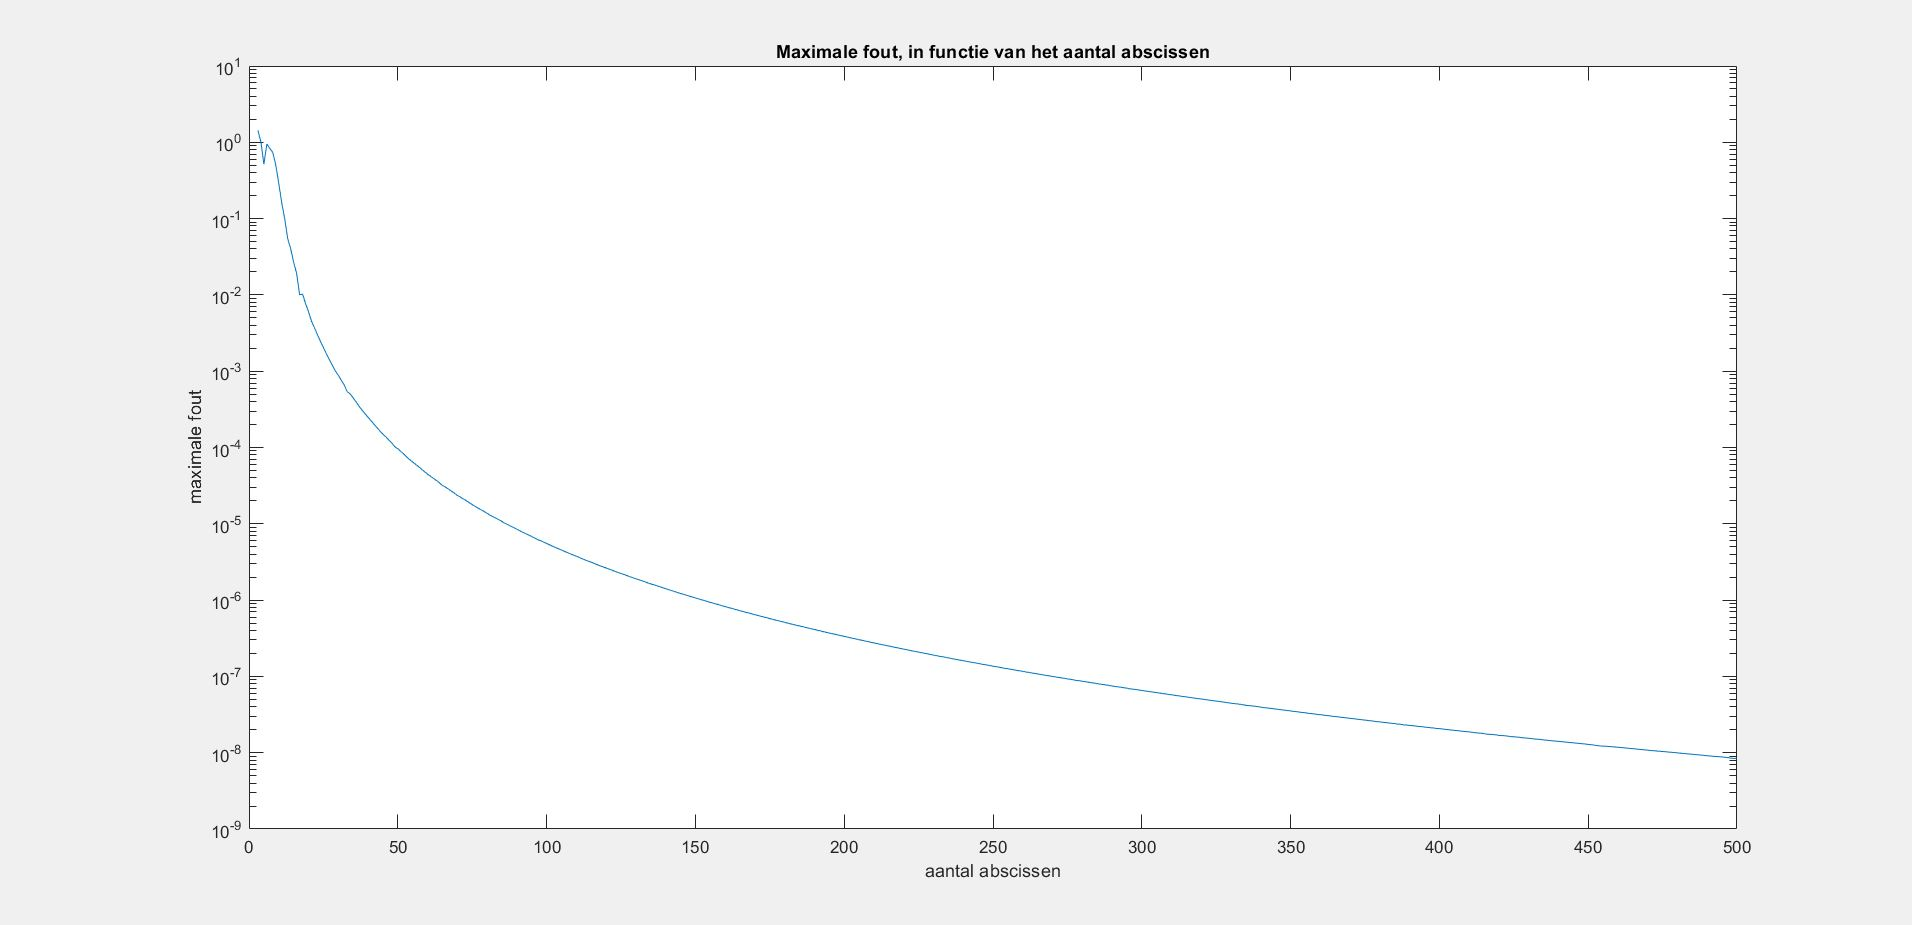
\includegraphics[width=\textwidth, height=0.3\textheight]{Excercise22AbsoluteErrorAbscis.JPG}
\end{figure}

\subsection{Deel 3 en Deel 4}
In deel 3 krijgen we x en y simpelweg door click() en evalueren we de x en y waarden samen. Als we op 4 willekeurige plaatsen klikken krijgen we figuur 9. We kunnen dan voor deel 4 bijvoorbeeld de striptekenfiguur Sidonia tekenen met deze functie. (Zie figuur 10). Om deze 2D spline-functies te evalueren hebben we gewoon aangenomen dat de abscissen (de t-waarden) equidistant zijn want we hebben geen functievoorschrift van de te benaderen functie.
\begin{figure}
\caption{Tekening met click()}
	\begin{minipage}{.5\textwidth}
		\centering
		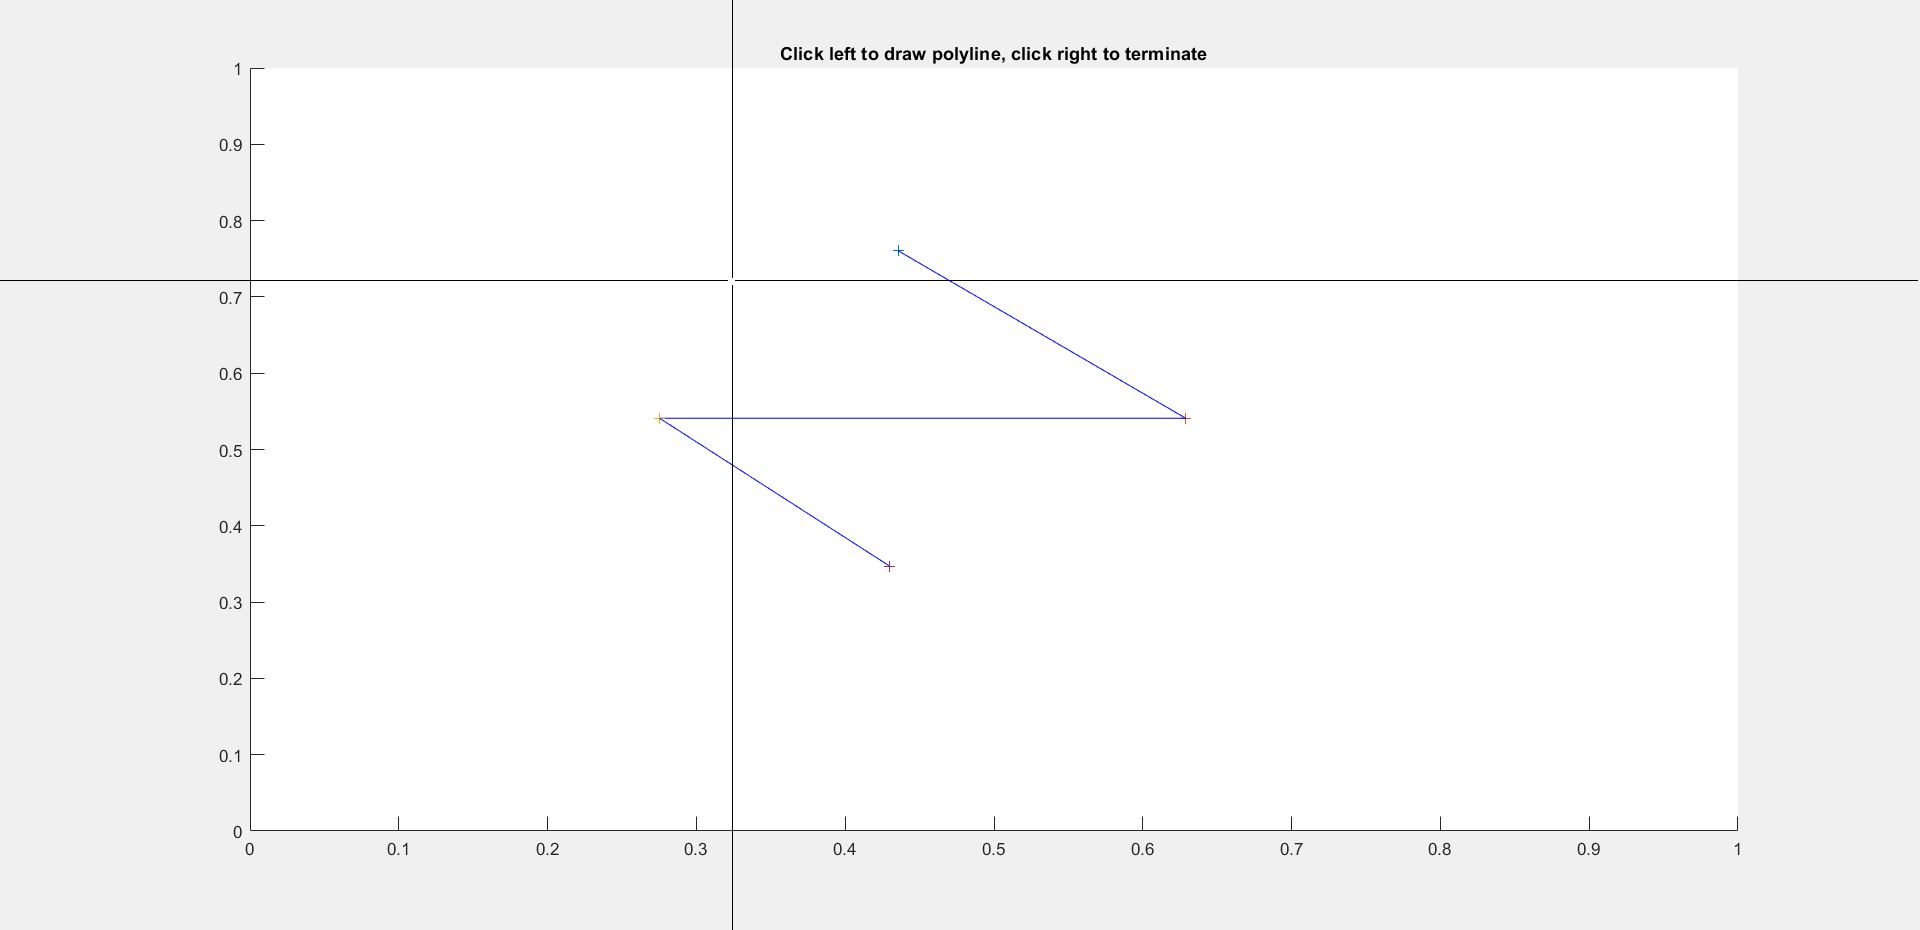
\includegraphics[width=\textwidth, height=0.2\textheight]{Excercise23.JPG}
	\end{minipage}
	\begin{minipage}{.5\textwidth}
		\centering
		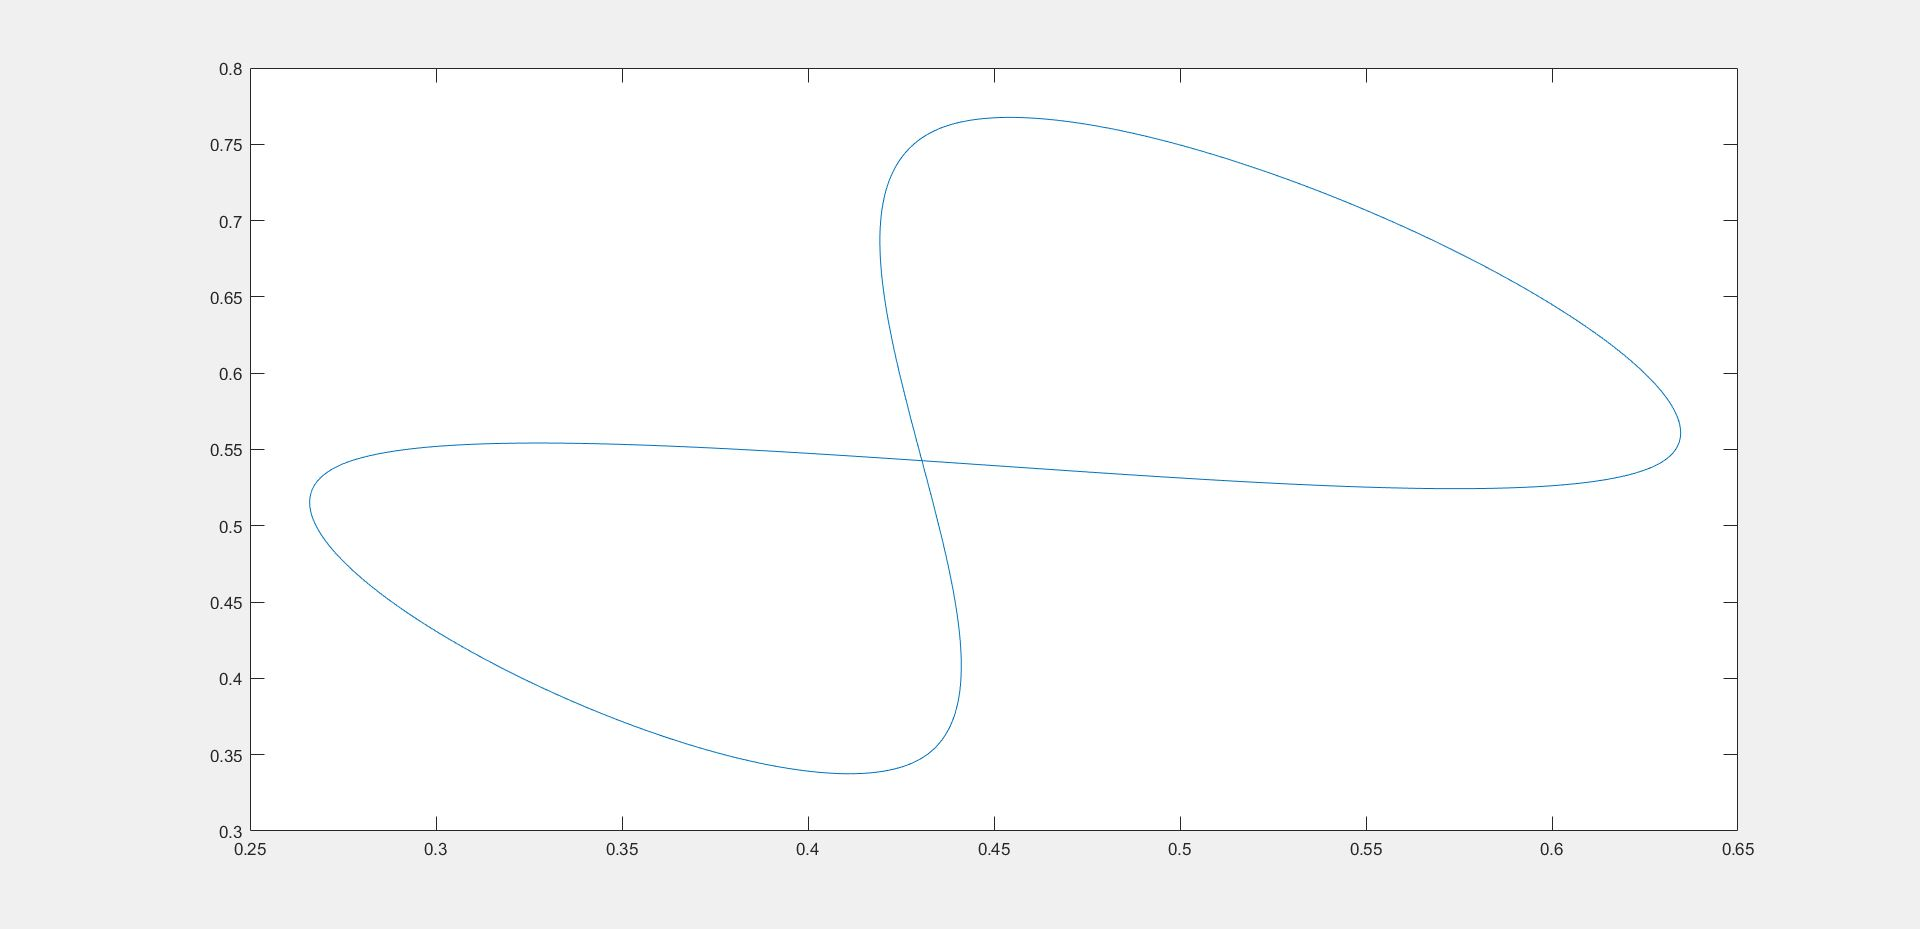
\includegraphics[width=\textwidth, height=0.2\textheight]{Excercise23Drawing.JPG}
	\end{minipage}
\end{figure}


\begin{figure}
\caption{Sidonia getekend via Splines}
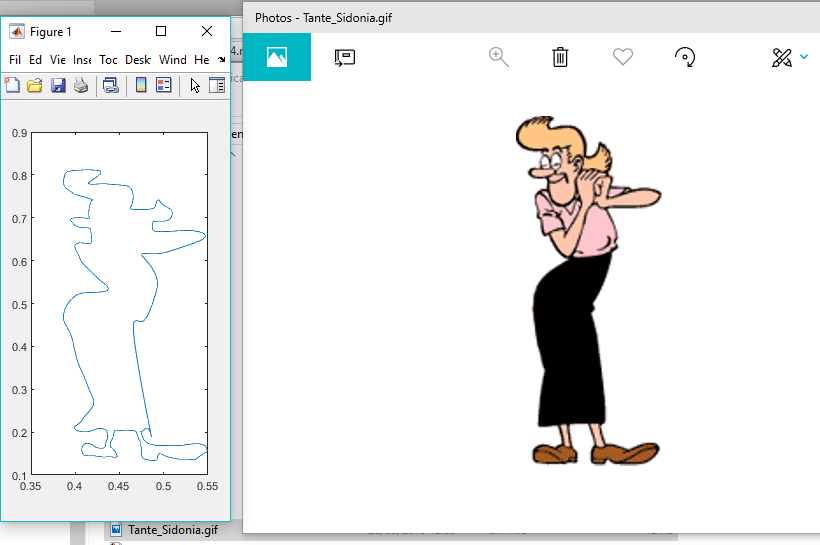
\includegraphics[width=\textwidth, height=0.3\textheight]{sidonia.png}
\end{figure}


\end{document}